\chapter{Introduction}

The modern electrical power grid is undergoing a profound structural and operational transformation, migrating from static, centralised architectures governed by electromechanical dynamics to highly variable, electronically-coupled decentralised networks. 
% The global electrical power infrastructure is transitioning from centralised, synchronous-machine-dominated architectures to networks integrated with decentralised, power-electronic-interfaced .
~This modernisation is driven by high-density deployment of Distributed Energy Resources (DERs) utilising inverter-based technologies with sophisticated power-electronic control algorithms, and non-linear demand profiles, such as Electric Vehicle (EV) fast-charging infrastructure.~The continuous expansion and technological evolution of the grid remain indisputably vital, serving as the foundational infrastructure required to sustain economic growth, industrial resilience, and decarbonization mandates across all sectors~\cite{peng2023power}.



\begin{figure}[!b]
\centering
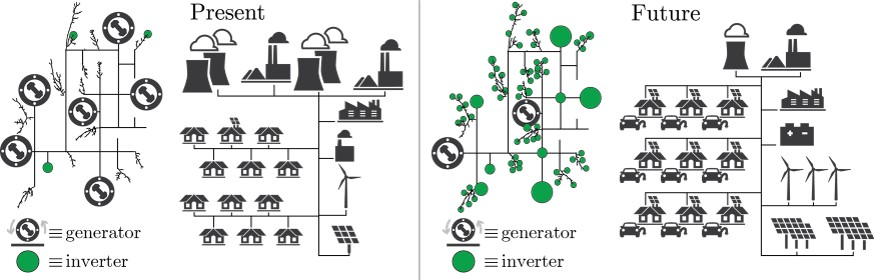
\includegraphics[scale=0.6]{images/chapter_1/Ch1F1.jpg}
\caption{Present and future power systems~\cite{peng2023power}}
\label{newgrid}
\end{figure}

Despite these rapid advancements in generation and load topologies, contemporary network protection remains fundamentally anchored largely to legacy, deterministic philosophies—legacy deterministic protection paradigms, specifically inverse-time overcurrent (ANSI 51) and impedance-based distance (ANSI 21) elements—which were explicitly designed for the high physical inertia and predictable short-circuit levels of synchronous machines \cite{ali2025power}. The power industry exhibits a pragmatic, stringent reluctance to overhaul these established paradigms, primarily because conventional relays have historically delivered exceptional dependability and security.~
% Completely replacing these philosophies introduces immense complexities in maintaining strict compliance with critical operational reliability standards, such as IEEE C37 and IEC 60255, while balancing economic constraints in complex, evolving networks.
The whole replacement of these established paradigms presents significant challenges in maintaining regulatory compliance with IEEE C37 and IEC 60255 standards.~However, to fully extract the technical and economic potential of these advanced generation and load technologies, and to safely facilitate the deployment of active smart grids and microgrids, the underlying protective philosophies must be aggressively updated \cite{brahma2009education}. 

% Confronting the vulnerabilities of legacy relaying—such as protective blinding, sympathetic tripping, and miscoordination caused by bidirectional, current-limited fault signatures—and proposing adaptive, communication-assisted, and data-driven protection frameworks forms the core technical mandate addressed throughout this thesis.




The imperative to aggressively upgrade medium and low-voltage distribution networks forms the critical next phase of this paradigm shift. Historically, distribution networks were engineered utilising simple, cost-optimised protection principles designed strictly for radial, unidirectional power flows where short-circuit currents were predictable and high in magnitude \cite{li2025gridforming}. However, this legacy framework is rapidly becoming obsolete due to the dense integration of bidirectional DERs alongside highly dynamic, non-linear load profiles. Compounding this complexity is the strategic deployment of localized clusters of distributed sources and loads operating as isolated cutsets or autonomous entities, formally defined as microgrids. These active microgrid architectures, capable of seamlessly transitioning between grid-connected and islanded operational modes, have evolved into an integral foundational framework of the modern decentralized power system.

Because the most acute protection vulnerabilities manifest at the grid edge under these dynamic conditions, this thesis directs its primary focus toward engineering advanced strategies to resolve the systemic issues plaguing modern active distribution networks and microgrids. This research addresses the existential need for a new generation of adaptive, high-fidelity, and data-driven protection architectures. By synthesising physics-informed transient characterisation with hierarchical control and machine learning paradigms, this thesis proposes protection solutions for next-generation autonomous grids.




\section{Background and Context}

For many years, existing protection and control applications have operated effectively within the framework of conventional grid architectures, and their performance has been exceptional. Nevertheless, the dynamics of modern power systems have shifted, creating new challenges for systems to uphold performance metrics \cite{srivastava2021review}.

\subsection{Evolving Topological Frameworks of Active Distribution Networks}

The fundamental topological shift in modern distribution networks—transitioning from classical radial architectures with strictly unidirectional power flow to dynamic, bidirectional networks—severely compromises legacy protection philosophies. Historically, radial distribution protection was predicated on unidirectional fault current paths with high-magnitude, predictable short-circuit infeeds. However, the aggressive proliferation of DERs completely fractures this assumption, requiring that, to effectively extinguish a fault and safely de-energise the affected zone, the protection scheme actively isolate the faulted component from all interconnected generation sources. Consequently, the cost-optimized distribution hardware of the past—reliant on localized magnitude sensing—is rendered technically obsolete due to inherent vulnerabilities like protective blinding, sympathetic tripping, and fuse-recloser miscoordination when subjected to bidirectional infeed. Resolving these bidirectional fault dynamics necessitates advanced interconnection protection frameworks, heavily relying on high-speed, peer-to-peer communication infrastructures like IEC 61850 GOOSE messaging to guarantee absolute fault selectivity \cite{mobashsher2025fault}.

% \begin{figure}[!b]
% \centering
% 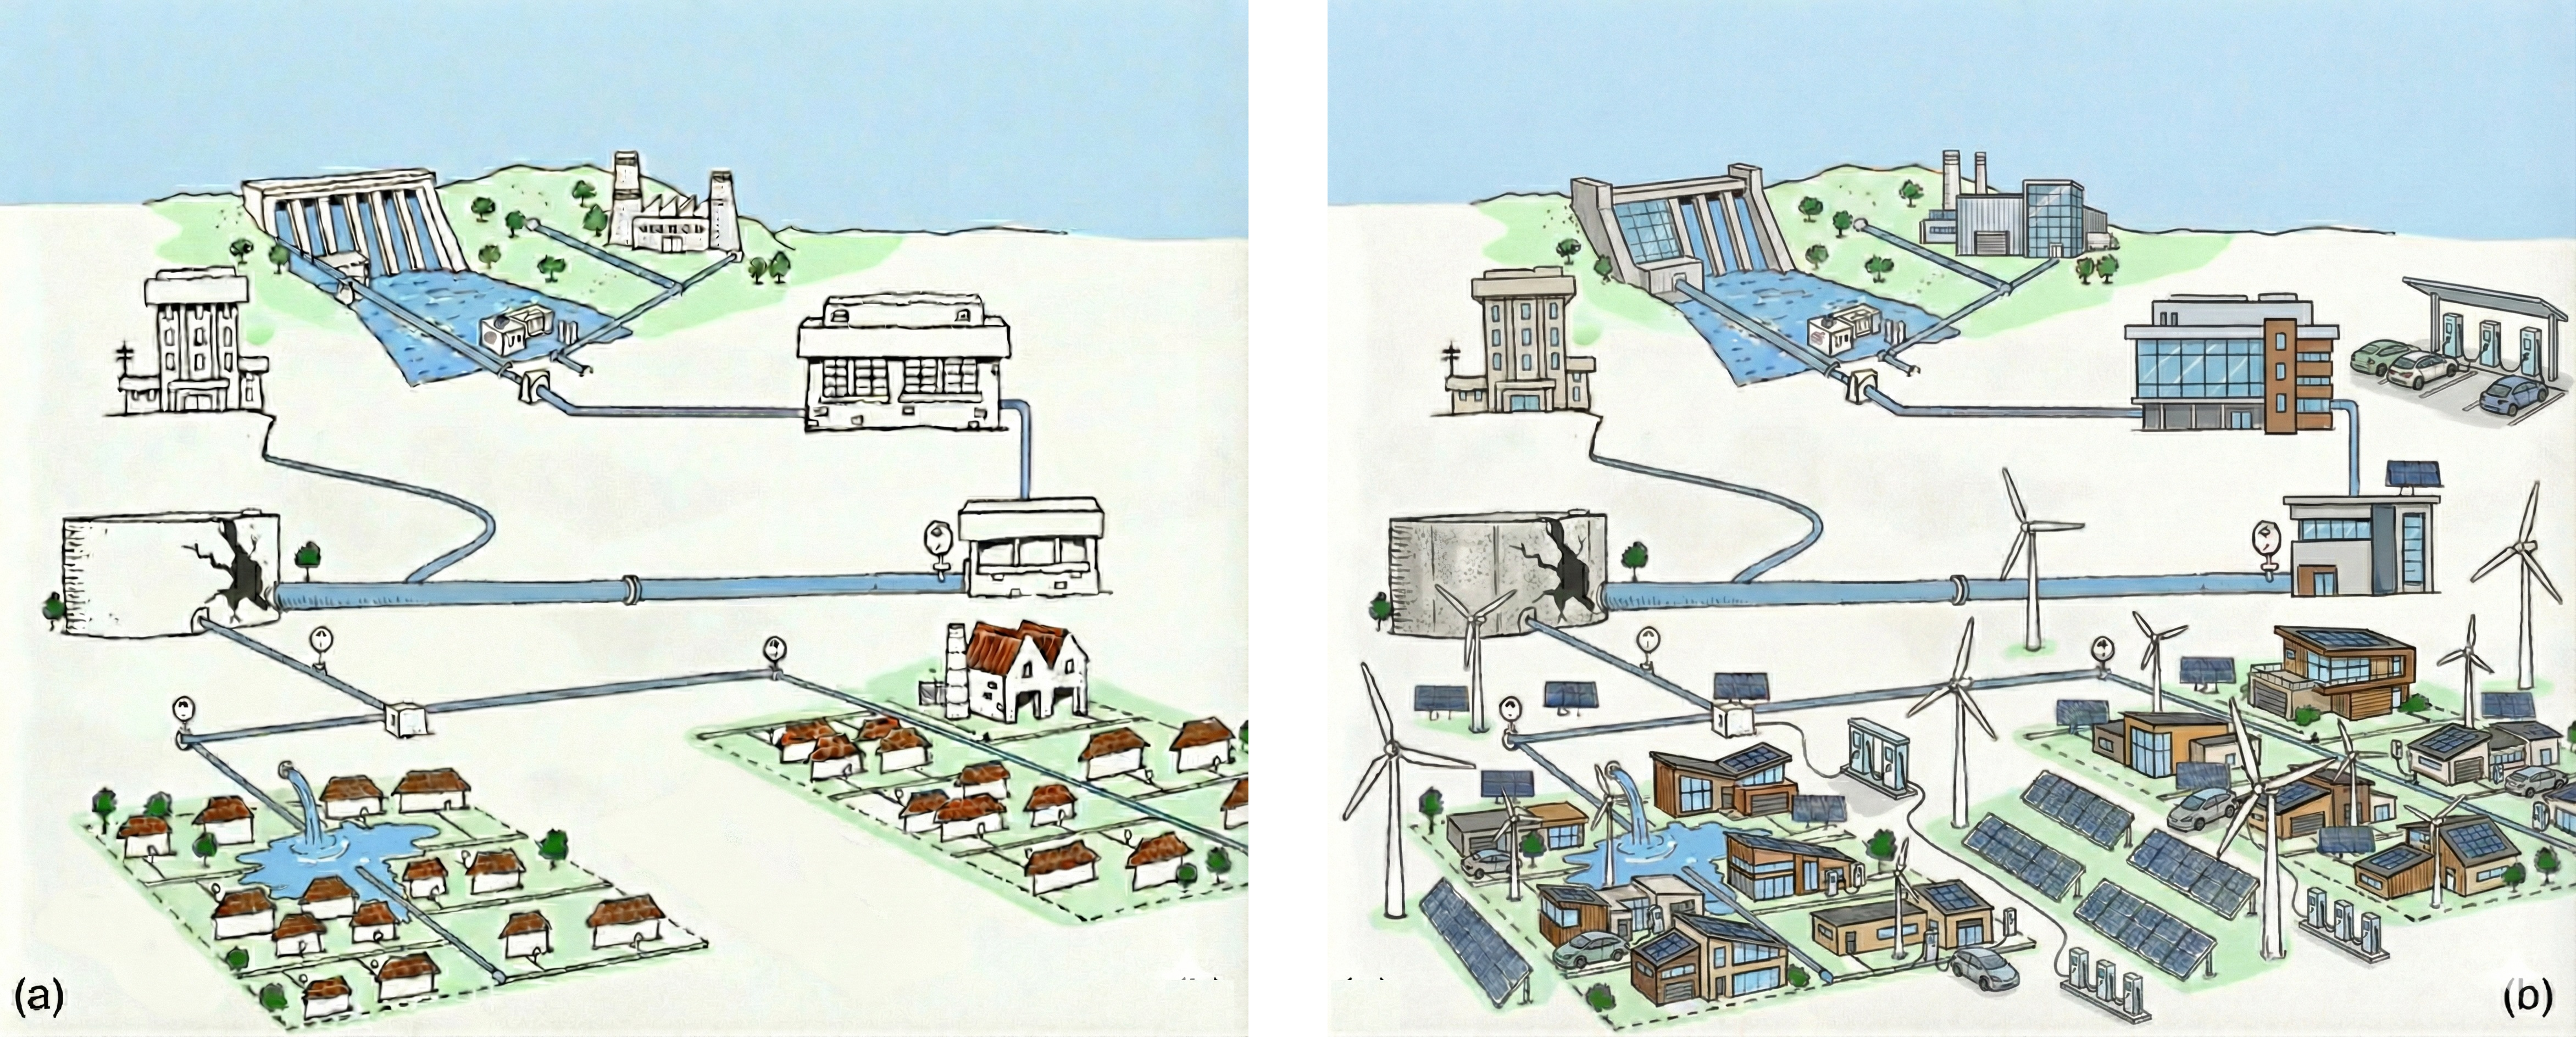
\includegraphics[scale=0.085]{images/chapter_1/DistributionFault.jpg}
% \caption{The fluid dynamics analogy comparing radial electrical grids to a single-reservoir water system}
% \label{newgridfluidflow}
% \end{figure}

\subsection{Fault Signature Characterization of Inverter-Based Resources}


The aggressive integration of advanced Distributed Generators into existing power networks has fundamentally shifted the generation profile from synchronous machine-based sources, governed by high physical inertia and slow electromechanical excitation controls, to fast, smart-controlled IBRs. The transient physical response of these converter-interfaced sources radically deviates from the deterministic "source behind impedance" characteristics of classical synchronous generators, which historically formed the foundational assumptions for legacy overcurrent and distance protection philosophies.
% Unlike synchronous machines whose fault response is inherently dictated by their sub-transient reactance, modern IBRs utilize rapid power electronic control loops to actively regulate and limit the magnitude and phase angle of fault currents, typically restricting outputs to near-rated values within milliseconds.
 IBRs' high-speed (sub-cycle) current limiters, which protect power electronic interconnections, typically cap fault current at 1.1 p.u. to 1.5 p.u., compared to 6.0 p.u. to 10.0 p.u. seen in Synchronous Machines. Furthermore, in the absence of specific advanced interconnection grid codes such as IEEE 2800, these smart inverters are frequently programmed to balance terminal voltages by actively suppressing negative-sequence current output during unbalanced phase faults. Additionally, because they act primarily as voltage-controlled, positive-sequence current sources, they inherently lack zero-sequence current contributions unless a specific grounding transformer topology is implemented, rendering conventional negative- and zero-sequence polarized elements (ANSI 67N/67G) ineffective due to suppressed sequence-current injection~\cite{sanati2024comprehensive}.


\subsection{Regulatory Landscape and Interconnection Compliance (IEEE 1547 / IEC 61727)}



Compounding the physical complexities of inverter fault signatures is the radical evolution of grid interconnection standards, which has fundamentally shifted the protective mandate from rapid local isolation to prolonged bulk grid support. Historically, legacy standards such as IEEE 1547-2003 mandated the immediate disconnection of DERs during abnormal conditions \cite{IEEE1547}. However, to preserve macroscopic grid stability under high renewable integration, continuous ride-through mandates have been aggressively adapted for active distribution networks via the revised IEEE 1547-2018 standard \cite{IEEE1547}. The modernized standard dictates a redefined "cease to energize" state during disturbances where inverters halt active power delivery but are actively permitted to exchange dynamic reactive power to support voltage recovery. While indispensable for transmission stability, this prolonged ride-through effectively blinds localised protection schemes and increases the allowable detection time for unintentional islanding. This regulatory evolution introduces a critical and severe operational conflict between bulk-grid support mandates (Ride-Through) and localised fault isolation speed.
% This regulatory shift creates a severe operational conflict: distribution system operators critically require fast source isolation to ensure safety and execute high-speed automatic reclosing without risking out-of-phase synchronization. 

Current industry mitigation practices remain fundamentally flawed; delaying upstream feeder trips degrades reliability, while implementing Direct Transfer Trip (DTT) schemes introduces prohibitive financial barriers and forces reliance on complex communication infrastructures.

\subsection{Impact of Reduced Rotational Inertia on Microgrid Fault Recovery}

\begin{figure}[!b]
\centering
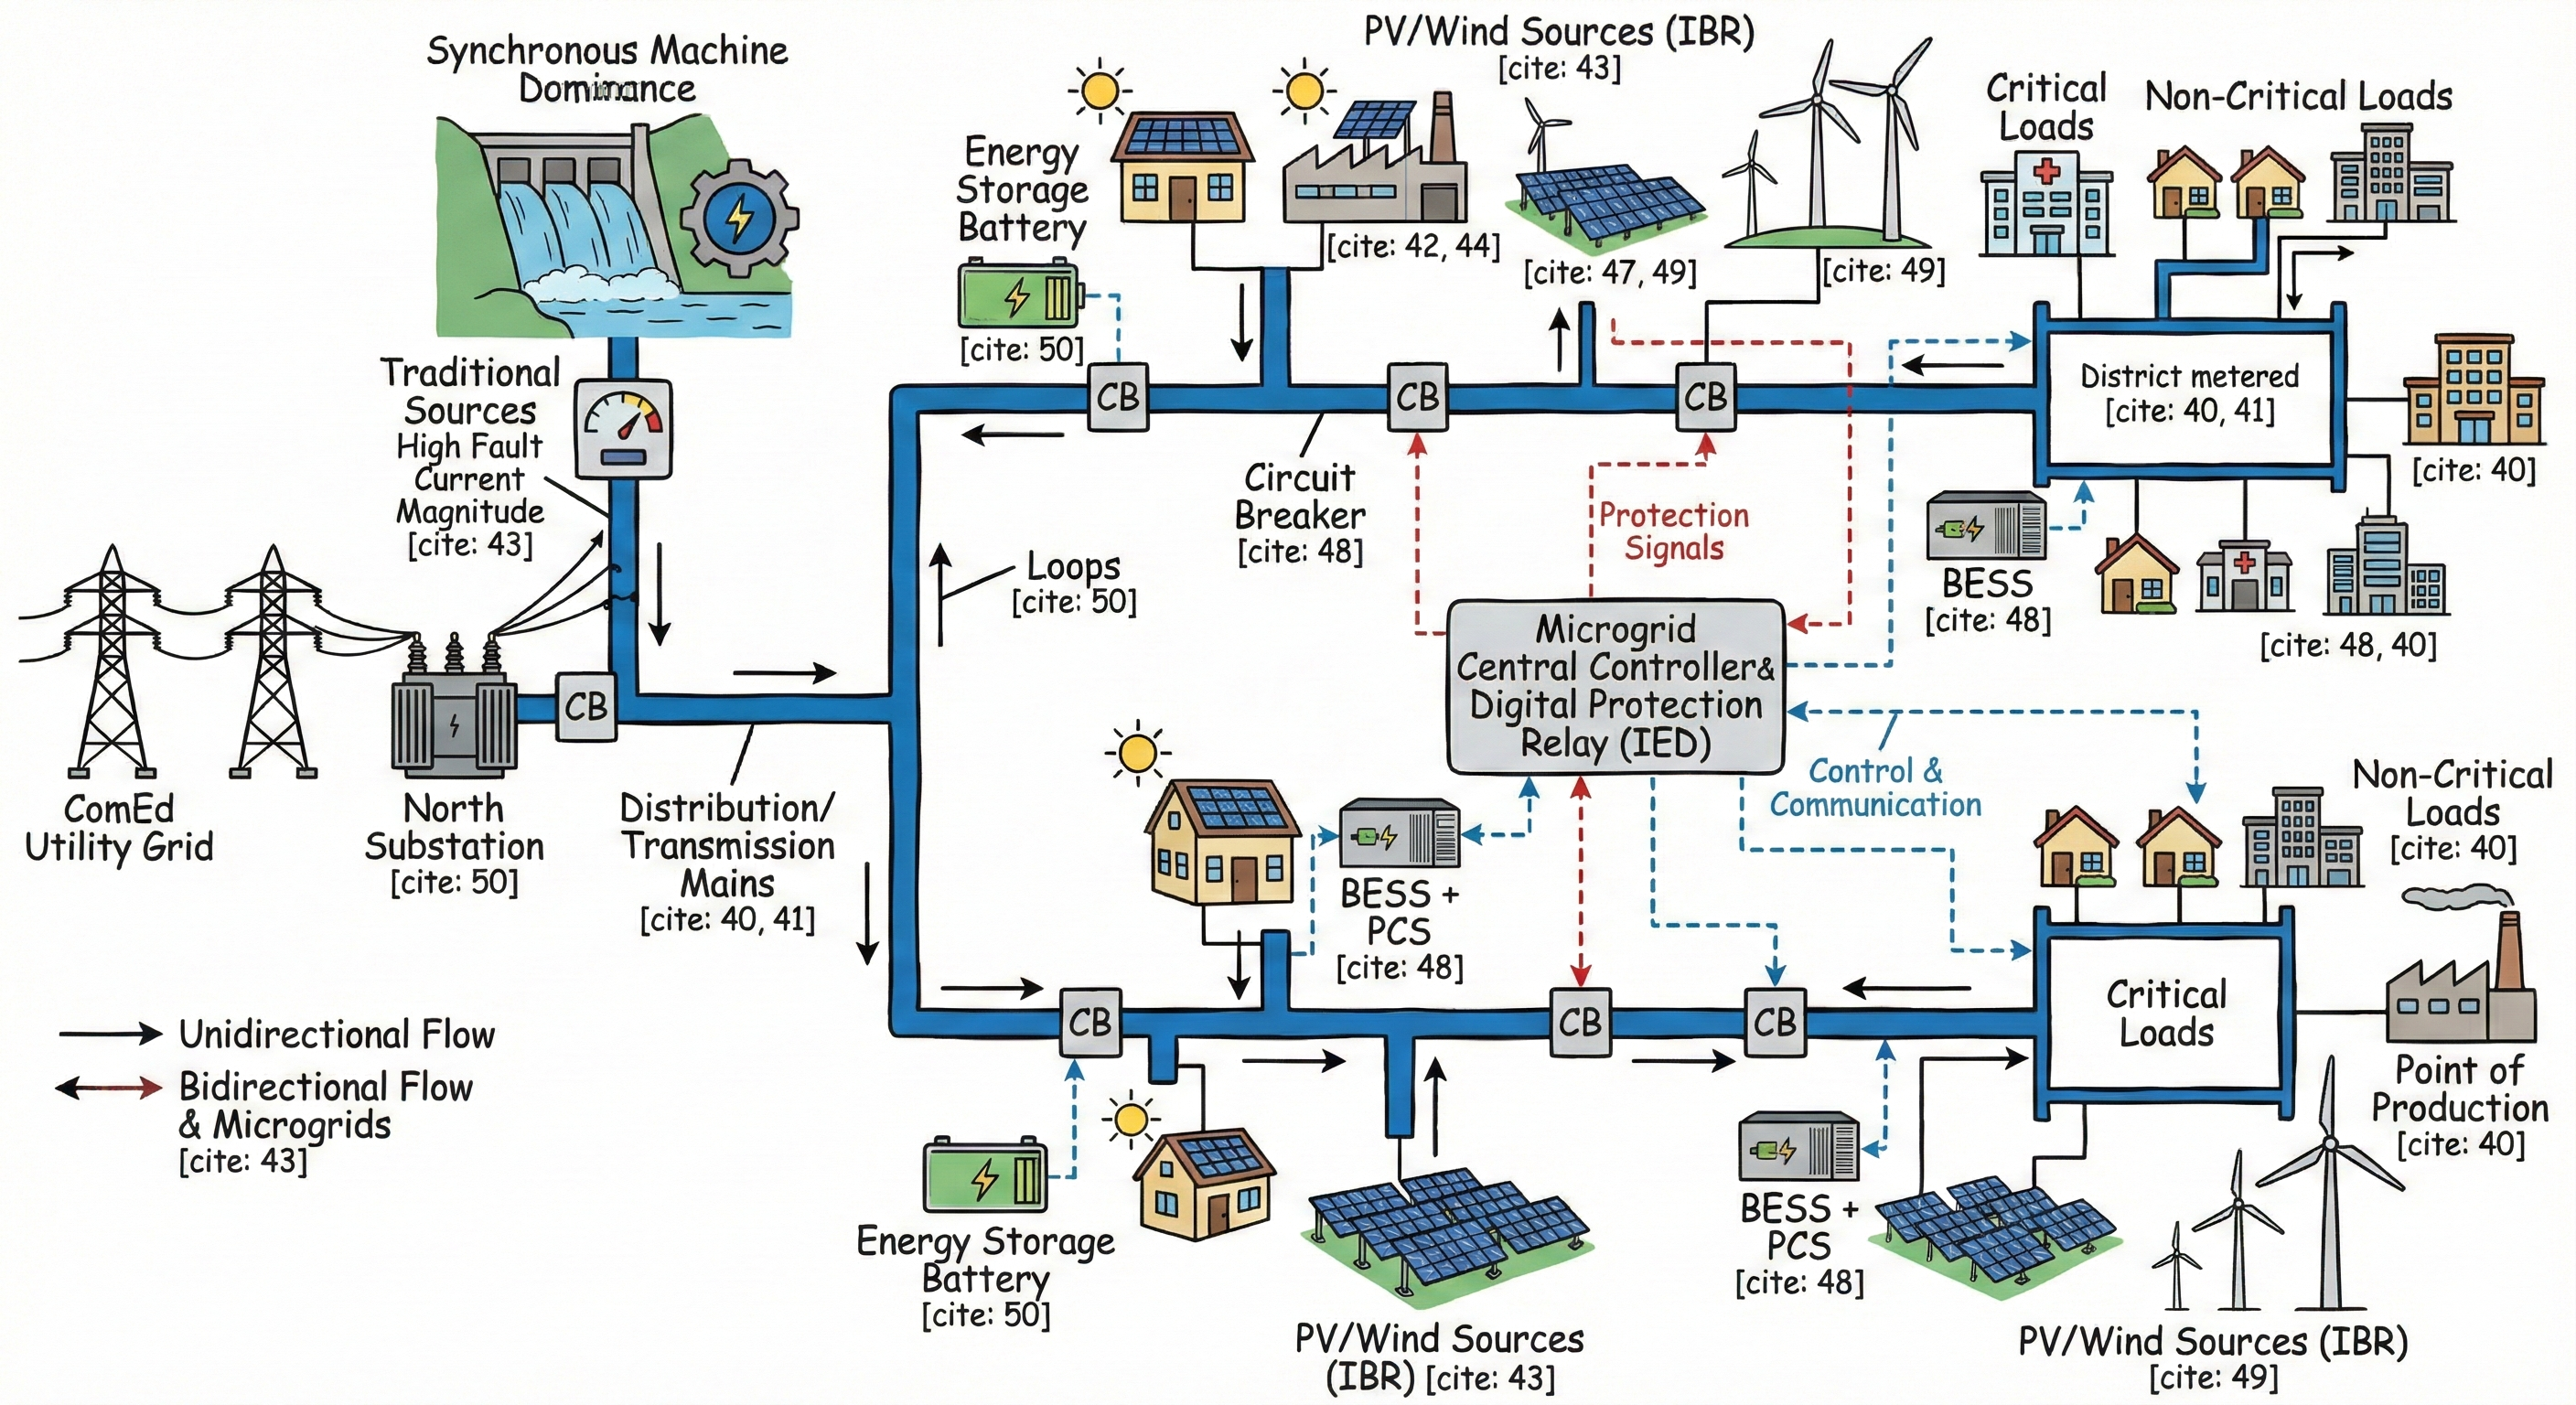
\includegraphics[scale=0.13]{images/chapter_1/Microgrid.png}
 \caption{The conceptual representation of a microgrid}
\label{microgridconcept}
\end{figure}


Transcending the localized boundary established by interconnection protection, the ultimate evolutionary phase of active distribution networks is the microgrid—a unified, controllable cluster of DERs and localized loads capable of operating either synchronized with the primary electrical power system (EPS) or autonomously in an islanded mode, figure \ref{microgridconcept} gives a conceptual representation. While offering unprecedented operational resilience, this paradigm shift introduces severe technical conflicts driven by the extreme variance in available short-circuit capacity during transitions between grid-connected and grid-isolated modes of operation. This topological uncertainty is critically compounded by the physical fault response of IBRs, which increasingly dominate modern islanded networks.



\section{Research Motivation}



\subsection{Physics-Based Modelling of DERs for Transient Response Characterisation under Unbalanced Faults}

A high-fidelity modelling requirement is necessary for the transient response characterisation of modern DERs, in which the fault current is not governed by the physical sub-transient reactance ($X''_d$) or the rotor's mechanical inertia. Modern IBRs are increasingly programmed to suppress negative-sequence currents ($I_2$) to prevent over-voltages on healthy phases. To characterise these transients, the High-Fidelity EMT modelling must move beyond the "Average Model" to the "Switching/Detailed Model". Inner Current Control Loops modelled in the $dq$-frame with a bandwidth exceeding 1 kHz to capture the high-frequency switching transients. The PLL's ability to track the grid frequency during a "Phase Jump" fault is critical. If the PLL loses synchronism, the IBR may trip prematurely, violating Fault-Ride-Through (FRT) requirements. Inclusion of the DC-link voltage dynamics to model the active/reactive power coupling during the fault period. Type IV (full-converter) wind turbines provide tightly controlled fault currents dictated entirely by grid-code-defined low-voltage ride-through (LVRT) curves while artificially suppressing negative-sequence injection. Conversely, Type III Doubly-Fed Induction Generators (DFIGs) exhibit highly non-linear and erratic fault responses during severe voltage dips due to the activation of hardware protection mechanisms like rotor crowbar circuits \cite{ieeereportImpactofinverterbased}.

% Comprehensive mathematical modelling, equivalent circuit formulations, and transient analysis characterizing specific IBR fault responses are systematically detailed in Chapter~2. Furthermore, these non-traditional sources inject highly unique transient signatures during short-circuit events. Solar photovoltaic (PV) generation facilities, for instance, exhibit a fault response strictly governed by their microprocessor controllers; they typically inject a brief sub-cycle transient due to the discharge of AC filtering components, before rapidly clamping the output to a restricted, symmetric current profile that effectively blinds traditional overcurrent elements. Wind generation sources introduce additional complexities depending on their mechanical and electronic topologies.






\begin{figure}[!b]
\centering
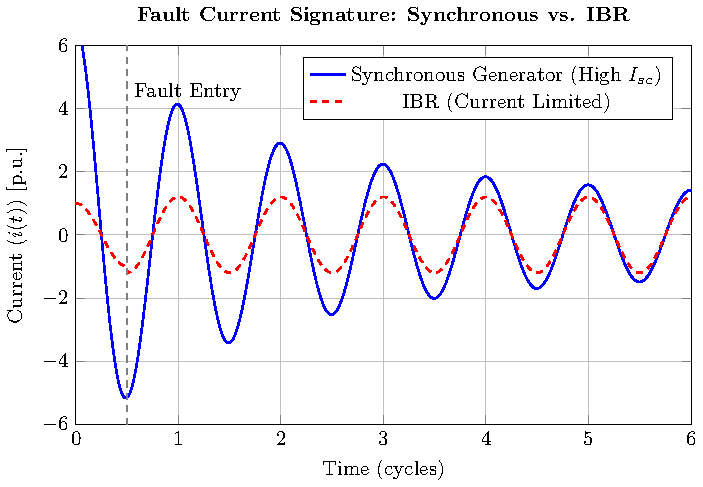
\includegraphics[scale=0.8]{images/chapter_1/Graphs2.pdf}
 \caption{Impact of IBR fault current.}
\label{Fig:ch_1_vieu}
\end{figure}

\subsection{Desensitisation and Mal-operation Risks in Legacy Protection Relaying Principles}

\begin{figure}[!b]
\centering
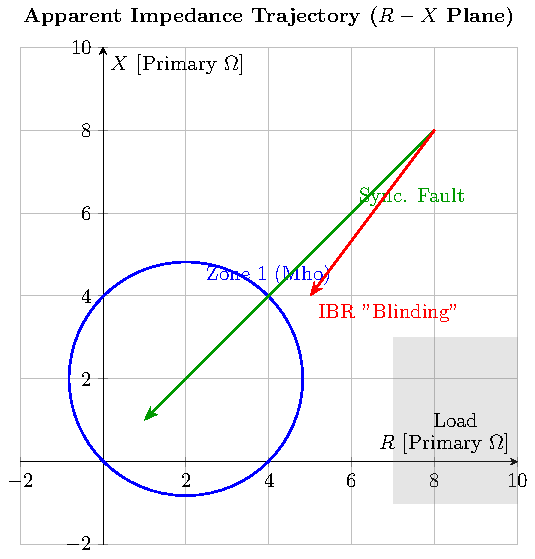
\includegraphics[scale=0.8]{images/chapter_1/Graphs1.pdf}
 \caption{The high sub-transient current causes the impedance to settle outside the trip zone.}
\label{Fig:ch_1_vieu}
\end{figure}

\begin{figure}[!b]
\centering
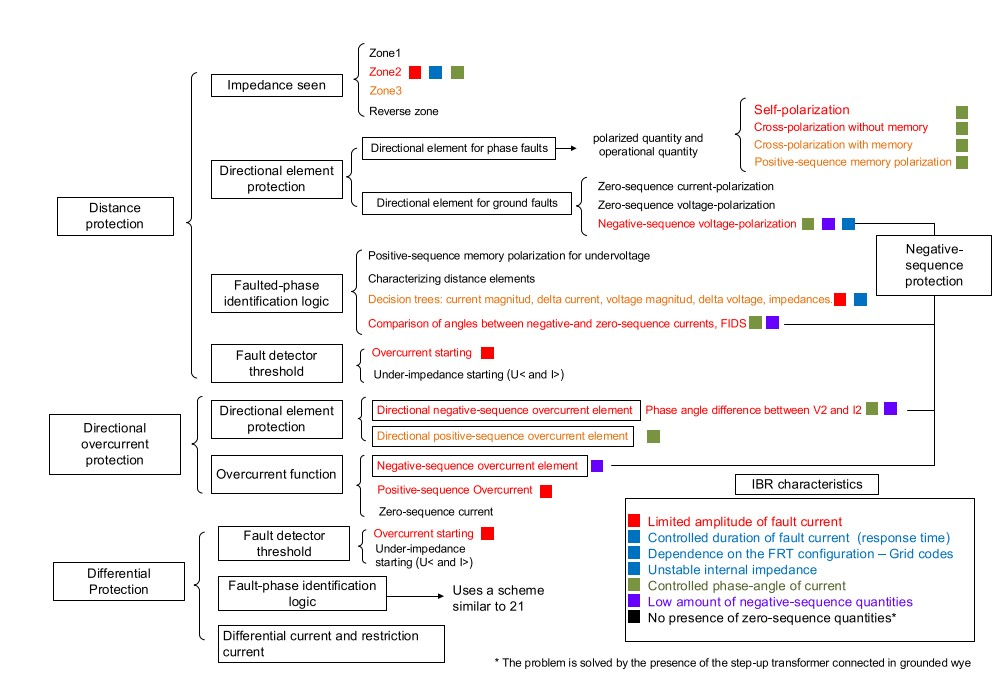
\includegraphics[scale=0.68]{images/chapter_1/Ch1F9.jpg}
\caption{Effects of IBR characteristics on the main protection functions.}
\label{protectionissus}
\end{figure}

\begin{figure}[!b]
\centering
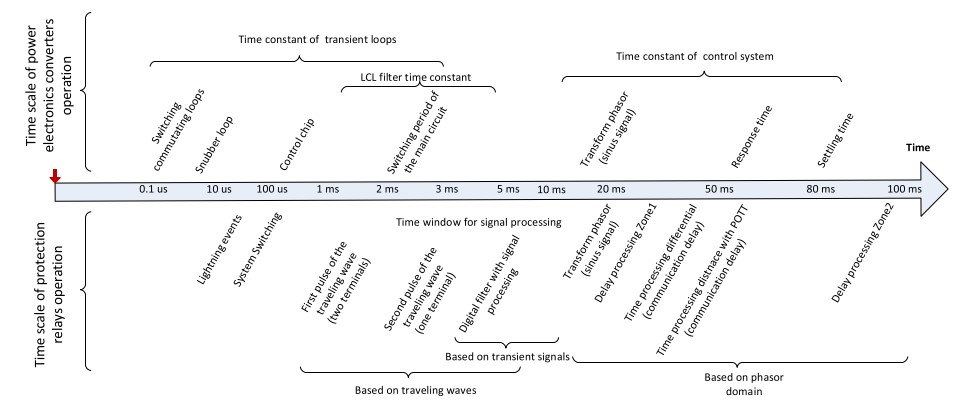
\includegraphics[scale=0.6]{images/chapter_1/Ch1F10.jpg}
\caption{Response time scale for the IBR operation and relays operation.}
\label{protectiontimes}
\end{figure}
However, despite their widespread industrial adoption, these conventional multi-function IEDs exhibit critical operational shortcomings when confronted with the dynamic transient behaviour of high-penetration IBR networks. The fundamental flaw lies in their reliance on simple RMS voltage calculations over a defined measurement window; this legacy signal-processing approach lacks the sensitivity, speed, and spatial resolution required to distinguish a genuine distribution fault from temporary, non-fault voltage sags. Furthermore, the stringent LVRT and dynamic reactive current injection mandates of modern grid codes actively antagonise these legacy relay functions. As the smart inverter actively injects reactive current to sustain terminal voltage and ride through the disturbance, the resulting current-limited, phase-shifted fault signature severely blinds the standard undervoltage and directional elements within the IED. Consequently, these multi-function relays fail to achieve the requisite balance of dependability and security, often resulting in delayed fault clearance, catastrophic miscoordination, or a complete failure to detect unintentional islanding within the mandated disconnection threshold.

The non-linear, converter-governed transient response of IBRs systematically degrades the efficacy of classical protection philosophies across all operational layers. IBRs can independently control reactive power injection ($Q$) during a fault. If the inverter control loop injects reactive power that shifts the current phase angle beyond the "Forward" sector of the relay, the directional element may perceive a forward fault as "Reverse." This leads to catastrophic mal-operation or the failure to isolate the faulted segment in a loop-configured or multi-source feeder. Distance relaying depends on the linear relationship between voltage and current to calculate the impedance to the fault ($Z = V/I$). The dynamic response of the inverter's voltage and current controllers makes the perceived impedance time-variant and non-linear. The "Apparent Impedance" seen by the relay during the sub-transient period deviates significantly from the actual line impedance. This results in Over-reach (tripping for faults outside the zone) or Under-reach (failing to trip for faults within the zone), compromising the fundamental selectivity of the protection scheme.
 

% Because IBRs actively limit fault current magnitudes, traditional inverse-time overcurrent relays (ANSI Device 51) suffer from severe protective blinding and under-reach. This deterministic failure propagates to directional overcurrent elements (ANSI Device 67) and distance relaying (ANSI Device 21), which are fundamentally compromised by the dynamic phase-angle responses and lack of standard sequence component injection mandated by modern grid codes during ride-through events as summaraized in figures \ref{protectionissus} and \ref{protectiontimes}. Beyond fault isolation, these factors severely complicate the detection of unintentional islanding conditions, masking the loss of the primary grid and defeating passive anti-islanding schemes, creating severe hazards for automatic reclosing practices.



\subsection{Protection Coordination Challenges in Bi-directional, Low-Inertia Power Networks}
 The rapid power electronic controllers of smart inverters actively clamp fault current contributions to near-rated continuous operational values,  in less than two cycles to protect internal semiconductor components, whilst dynamically altering fault current phase angles and frequently suppressing critical negative- and zero-sequence current components.
This abrupt, artificial suppression of fault magnitude, coupled with bidirectional fault flows originating from multiple distributed sources, fundamentally invalidates deterministic, magnitude-sensing legacy protection philosophies,. Specifically, it renders traditional time-overcurrent relays (IEEE Device 51) and classical distribution fuses technically obsolete; operating under these non-linear, converter-governed fault signatures subjects the network to severe protective blinding, excessively prolonged fault clearing times (e.g., increasing from sub-second operation to several seconds), and a catastrophic loss of spatial selectivity, Furthermore, the active suppression of unbalanced current injections by inverters fundamentally cripples traditional sequence-based unbalanced fault and directional detection elements.
\subsection{Balancing  speed requirements and cost constraints for microgrid protection}
Consequently, securing the modern microgrid dictates an urgent and absolute paradigm shift from static, deterministic methodologies to a highly adaptive, communication-assisted, and multi-domain protection architecture capable of functioning independently of macroscopic fault current availability.
\subsection{Limitations of Standard Interconnection Protection Relay logics for IBRs}

Building upon the systemic vulnerabilities identified across localized protective devices, the ultimate boundary of grid security in active distribution networks lies at the Point of Common Coupling (PCC) or Point of Interconnection (POI) through dedicated interconnection protection. Interconnection protection serves as the critical safeguard established between the utility grid and the Distributed Generation (DG) or IBR facility. Its primary technical mandate is to securely govern parallel operations, isolate the grid from DG-induced abnormalities, and safely disconnect the generation facility during severe utility-side faults or unintentional islanding conditions, while strictly adhering to modern grid codes such as IEEE 1547 and IEEE 2800 \cite{ieeestandard2022}. In contemporary practice, this protective boundary is enforced utilizing advanced multi-functional digital relays, or Intelligent Electronic Devices (IEDs), manufactured by prominent industry leaders. These digital relays typically synthesize a suite of deterministic, RMS-based elements to monitor the interconnection—predominantly relying on undervoltage (ANSI Device 27), overvoltage (ANSI Device 59), under/over-frequency (ANSI Device 81O/U), directional power (ANSI Device 32), and rate-of-change-of-frequency (ROCOF) elements to initiate trip decisions.

\subsection{Necessity of AI/ML for Fault Detection in Non-Deterministic Microgrid Environments}
Finally, the proliferation of high-resolution digital fault data has catalyzed the deployment of Artificial Intelligence and Machine Learning (AI/ML) frameworks. Algorithms such as Support Vector Machines (SVM), decision trees, and deep neural networks are increasingly utilized for real-time dynamic setting optimization and highly accurate fault classification. These data-driven models rapidly identify fault types and locations in 100\% inverter-based microgrids, offering an operational resilience that effectively transcends the limitations of deterministic mathematical models \cite{ml_microgrid_2024}.

\section{Literature review of advancements in protection principles and applications}

To counteract the fundamental protection vulnerabilities introduced by IBRs and bidirectional microgrid topologies, contemporary research has proposed a multitude of advanced, non-deterministic protection strategies. These methodologies deliberately pivot away from static magnitude-sensing toward adaptive, multi-variable, and data-driven algorithms capable of securing the grid edge.

\subsection{Industrial maturity of dynamic settings and adaptive principles in modern IEDs}
Recognizing the extreme variance in fault current availability between grid-tied and islanded modes, adaptive relaying architectures continuously monitor real-time network parameters—such as topology reconfigurations and DER connection statuses. By utilizing centralized microgrid controllers, these systems dynamically recalculate and deploy optimal protection settings to intelligent electronic devices (IEDs), ensuring persistent selectivity and coordination without manual intervention \cite{patel2023hardware}.

\subsection{Limitations of Sequence-Component Based Directional Discrimination}
The active suppression of sequence components and the manipulation of fault phase angles by IBR controls have severely crippled conventional directional overcurrent relays (ANSI 67). To restore directionality, recent literature emphasizes voltage-based directional elements that leverage the phase angle relationships of superimposed or pre-fault voltage-current vectors, effectively bypassing the current-limiting blinding effects of the inverters \cite{seq_directional_2024}.

Furthermore, reactive power directional protection—specifically utilizing the Equivalent Voltage Polarizing Method and V–I ellipse trajectory tracking—has emerged as a robust technique. These methods determine fault direction by analyzing transient energy flows and phase-plane trajectories, remaining highly secure even under heavily constrained, bidirectional fault current scenarios \cite{energy_directional_2023}.

\subsection{IEC 61850 based GOOSE messaging  in modern industry IEDs}

Achieving absolute spatial selectivity and mitigating sympathetic tripping in dense microgrid architectures necessitates high-speed, peer-to-peer data exchange. Modern communication-assisted schemes heavily leverage the IEC 61850 standard. By utilizing Generic Object-Oriented Substation Events (GOOSE) messaging and synchrophasor-based differential algorithms, these systems execute sub-cycle directional interlocking and localized fault isolation with latencies well below the critical clearing times demanded by modern grid codes \cite{aftab2018performance}.

\subsection{Real-time Simulation and Prototyping Trends}

\begin{itemize}
\item Absence of Universal, Scalable Protection Architectures.
\item LVRT vs. Genuine Fault Discrimination Failures.
\item Inadequacy of Deterministic RMS-Based Relaying.
\item Discrimination of temporary faults and Anti-Islanding Detection Conflict.
\end{itemize}

\subsection{Emerging Trends: Digital Twins and Physics-Informed Neural Networks (PINNs)}
Despite the continuous deployment of adaptive numerical relays and communication-assisted coordination frameworks, fundamental research gaps persist in the protection of modern active distribution networks. A primary deficiency is the lack of universal protection schemes capable of securely accommodating mixed DER topologies. Furthermore, a profound technical conflict exists regarding the difficulty in differentiating genuine network faults from LVRT behaviour during grid voltage dips.

% % Requires: \usepackage{array}
% \begin{table}[!h]
%     \centering
%     \caption{Critical Research Gaps and Technical Motivations in Active Distribution Network Protection}
%     \label{tab:placeholder_label}
%     \begin{tabular}{|>{\raggedright\arraybackslash}p{0.32\textwidth}|>{\raggedright\arraybackslash}p{0.60\textwidth}|}
%         \hline
%         \textbf{Fundamental Research Gap} & \textbf{Technical Implications and Motivation} \\
%         \hline
%         Absence of Universal, Scalable Protection Architectures &
%         Current engineering relies on bespoke, topology-specific designs that fail to scale. The heterogeneous integration of mixed DERs—including conventional synchronous machines, Type III DFIGs, and Type IV full-converters—introduces highly non-linear, transient fault signatures that systematically collapse classical time-graded coordination intervals. \\
%         \hline
%         LVRT vs. Genuine Fault Discrimination Failures &
%         Grid codes (e.g., IEEE 1547-2018, IEC 61400-21) mandate that Inverter-Based Resources (IBRs) sustain connection and inject dynamic reactive current during undervoltage events. This controlled response alters the voltage-current phase angle and suppresses fault magnitude, effectively blinding conventional distance (ANSI 21) and directional overcurrent (ANSI 67) elements. \\
%         \hline
%         Inadequacy of Deterministic RMS-Based Relaying &
%         Conventional multi-function Interconnection Protection Relays (IPRs) rely heavily on simple Root Mean Square (RMS) undervoltage calculations (ANSI 27). This legacy signal processing fundamentally lacks the transient spatial resolution required to differentiate between a fault-induced voltage sag and a non-fault depression (e.g., severe motor starting or transformer magnetic saturation). \\
%         \hline
%         LVRT and Anti-Islanding Detection Conflict &
%         Prolonged ride-through mandates actively antagonize rapid anti-islanding mechanisms. Under high DG penetration, the active regulation of voltage and frequency by inverter controls expands the Non-Detection Zone (NDZ), defeating passive rate-of-change-of-frequency (ROCOF) schemes and jeopardizing the mandatory 2.0-second disconnection threshold. \\
%         \hline
%         \end{tabular}
% \end{table}


\section{Research Objectives}

To systematically dismantle the operational barriers identified in the research gap, this thesis engineers a robust, topology-agnostic protection architecture capable of securing active distribution networks under extreme fault current variance. 
The specific research objectives are meticulously defined as follows:
 
\subsection{Objective 1 : To Develop Fault-Resilient Adaptive Interconnection Protection Logics for IBR-Dominated Distribution Networks}
This architectural synthesis logically commences at the network perimeter: the PCC. Before internal stability can be managed, the microgrid boundary must be decisively secured against utility-side disturbances without succumbing to the operational paradox introduced by modern grid codes. Specifically, ride through requirements by IEEE 1547-2018. Operating under these non-linear, converter-governed fault signatures critically blinds traditional undervoltage elements (27), and fundamentally confounds sequence-polarised directional overcurrent relays (67). To overcome this deterministic protective blinding, the proposed interconnection framework abandons legacy RMS-based magnitude sensing in favor of high-speed instantaneous time-domain sampling. By utilising geometric extraction of a Space Phasor Model (SPM)—specifically analysing the tilt angle and eccentricity of the voltage locus—the proposed Enhanced Voltage Protection Module (EVPM) accurately distinguishes genuine fault-induced voltage sags from mandatory LVRT reactive current injections. This highly adaptive transient spatial resolution ensures absolute fault selectivity at the PCC, rapidly isolating the microgrid to prevent catastrophic out-of-phase synchronisation events caused by uncoordinated upstream utility automatic reclosing schemes.

\subsection{Objective 2 : Hierarchical Microgrid Protection}
Hierarchical Protection handles the coordination (communication layer). Following the definitive isolation of the PCC from utility-side disturbances, the protective architectural focus shifts strictly to the internal microgrid boundary. Operating under these artificially suppressed, converter-governed fault signatures fundamentally invalidates single-strategy, classical time-current coordination methodologies. To definitively resolve this topological vulnerability, this research engineers a rigorous, hierarchical Four-Level Protection Architecture. At the foundational tier (Level 0 - Local Element Layer), the architecture explicitly abandons static magnitude-sensing in favour of decentralised, autonomous voltage-restrained and voltage-controlled overcurrent relays (IEEE Devices 51VR and 51VC). By dynamically adjusting the overcurrent operating thresholds based on localised voltage depressions, these adaptive elements ensure highly sensitive fault detection even when IBRs strictly limit fault current availability. However, localised voltage restraint inherently fails to resolve the severe spatial selectivity loss caused by bidirectional fault currents originating from multiple distributed generation sources within dynamic microgrid topologies. Therefore, the architecture integrates a supervisory tier (Levels 1 and 2) that synthesises high-speed communication infrastructure to enforce peer-to-peer coordination and to supervise microgrid controllers. This layer mandates the deployment of IEC 61850 GOOSE messaging to precisely communicate the direction of fault currents and execute communication-based line current differential protection (IEEE Device 87L) alongside high-speed directional interlocking schemes. By bypassing the inherent delays of magnitude-based time-grading, this synthesis guarantees absolute spatial selectivity, eliminates sympathetic tripping, and ensures stable microgrid recovery across all operational boundaries.

% The high-noise, highly distorted transient fault signatures of IBR networks exceed the boundaries of deterministic curve-fitting algorithms proposed for IPRs.

The non-linear, stochastically distorted transient signatures of IBR-dominated networks transcend the mathematical constraints of deterministic signal-processing algorithms. To ensure robust fault classification regardless of aliasing or sub-Nyquist sampling variances, the architecture integrates Transform-Domain Deep Convolutional Neural Networks (CNNs) to process the 2-D and 3-D spatial representations of the SPM, autonomously executing dynamic feature selection and fault classification. This multi-layered approach moves beyond mere fault detection, establishing a comprehensive, adaptive defense system capable of securing the dynamic microgrid against extreme topological and short-circuit variances.
\subsection{Objective 3: Data-Driven Paradigms for advanced Microgrid protection}
AI/ML handles the classification (local intelligence) where current sensors provide noisy or insufficient data.
Ultimately, the highly non-linear, transient-heavy fault signatures intrinsic to IBR-dominated networks systematically exceed the mathematical boundaries of conventional deterministic curve-fitting algorithms proposed for IPRs. Relying on simplified physical circuit models and static settings inevitably results in severe protective blinding, delayed operation, and the inability to securely distinguish between genuine faults and high-noise, non-fault transient events. To definitively overcome these deterministic limitations and transcend the constraints of conventional signal processing, the proposed protective architecture integrates a sophisticated Artificial Intelligence framework. Instead of discarding transient signatures, the architecture mathematically transforms raw, high-speed time-domain measurements into 2-D and 3-D spatial representations via the Space Phasor Model (SPM). Processing these multi-dimensional representations through Transform-Domain Deep Convolutional Neural Networks (CNNs) explicitly leverages deep representation learning. This allows the neural network to autonomously execute dynamic feature selection and precise non-linear fault classification, achieving absolute accuracy entirely independent of traditional fundamental power-frequency sampling constraints. By synthesising physics-informed spatial modelling with deep learning, this multi-layered approach moves beyond mere magnitude-based fault detection, establishing a comprehensive, adaptive defence system capable of securing the dynamic microgrid against extreme topological uncertainties and severe short-circuit variances


\section{Key Contributions}

The execution of the identified objectives yields several distinct, state-of-the-art contributions to the field of power systems protection:


\subsection{Development of adaptive protection logics for Multifunctional Interconnection Protection Relays (C1)}.

Formulates a robust detection algorithm that remains immune to the non-linear, current-limited fault signatures of IBRs, satisfying both IEEE 1547 and local FRT requirements. This is executed through distinct logic modules. \\
\textbf{Algorithms for Multi-Functional Adaptive Interconnection Protection}.
 \begin{itemize}
        \item Novel Fault Phase Selection Logic. 
        \item Enhanced Voltage Protection Module (EVPM).
        \item Adaptive Reclosing Coordination.
        \item Advanced Islanding Detection.
        \item Dynamic Feature Selection and Settings Groups.
    \end{itemize}



% \textbf{Algorithms for Multi-Functional Adaptive Interconnection Protection}
% The primary objective within this domain is to redefine interconnection protection to securely accommodate the current-limited, non-standard fault responses of IBRs. The proposed architecture fundamentally reorientates the protection paradigm from static overcurrent coordination to dynamic fault detection based on precise physical signal footprints.~Development of a Space Phasor Model (SPM) framework that bypasses RMS sensing to resolve the Inadequacy of Deterministic Relaying (Gap 3).~By analyzing regulated network parameters—specifically instantaneous voltage, frequency, and real/reactive power responses—the Enhanced Voltage Protection Module (EVPM) utilizes instantaneous time-domain sampling to resolve the LVRT vs. Genuine Fault Discrimination paradox (Gap 2).

% A foundational advancement in this approach is the transition from traditional RMS measurements to high-speed instantaneous time-domain sampling. RMS-based relays are inherently vulnerable during unintentional islanding events, where severe frequency drifts and waveform distortion corrupt measurement windows. Instantaneous sampling provides a frequency-independent protective layer, ensuring deterministic operation under volatile conditions. This is executed through distinct logic modules:

\subsubsection{Novel Fault Phase Selection Logic}
To bypass conventional sequence-component logic—which is frequently compromised by IBR negative-sequence current suppression—this module utilizes a Space Phasor Model (SPM) derived from instantaneous three-phase voltages. By mapping geometric transformations of the voltage locus from a nominal circle to a fault-induced ellipse, the logic precisely extracts tilt angle and eccentricity parameters to classify fault phase signatures.
\subsubsection{Enhanced Voltage Protection Module (EVPM)}
This logic executes multi-layer analysis combining extracted voltage parameters with reactive power signatures. This synthesis facilitates seamless coordination with mandatory LVRT grid codes (e.g., IEEE 1547-2018), ensuring highly selective fault isolation without violating continuous operation mandates.
\subsubsection{Adaptive Reclosing Coordination}
The EVPM algorithm tracks voltage dip staging to coordinate robustly with upstream feeder reclosers (ANSI Device 79), ensuring rapid isolation of DG sources during temporary faults to prevent out-of-phase reclosing sequences.
\subsubsection{Advanced Islanding Detection}
To mitigate non-detection zones during power-balanced islanding conditions, the architecture integrates advanced signal processing methodologies, such as transform-domain techniques, to extract high-frequency harmonic transient features indicative of grid loss.
\subsubsection{Dynamic Feature Selection and Settings Groups}
The system employs adaptive feature extraction to dictate setting group selections based on real-time topological states, ensuring instantaneous adjustment of Interconnection Protection Relay (IPR) trip boundaries.

\subsubsection{Validation Framework}
Comprehensive PSCAD-Based Verification of Protective Relaying Stability. Provides a high-fidelity validation of the proposed algorithms against a wide range of DER penetration levels and different network topologies.

    
\subsection{Synthesis of Multi-Layered Hierarchical Protection Architectures for AC Microgrids (C2)}

% The fulfilment of these research objectives establishes a novel, magnitude-agnostic paradigm that systematically resolves the identified gaps in IBR protection.

%\textbf{Key Thesis Contributions}

Establishes a communication-assisted coordination strategy that dynamically adjusts relay settings in real-time based on the transition between grid-connected and islanded operational modes. This framework strategically synthesises decentralised and centralised adaptive logics.\\

     \textbf{Protection architectures for microgrids}.
    \begin{itemize}
        \item Adaptive Multi-Tier Logic.
        \item Integrated Flexible Load Management for EV loads.
        \item Communication-Based Differential Schemes.
    \end{itemize}
        \begin{itemize}
            \item Hardware-in-the-Loop (HIL) Validation
        \end{itemize}




% \subsection{Protection architectures for microgrids}
% Engineering a four-level supervisory framework to resolve the Absence of Universal Protection Architectures (Gap 1). Addressing the extreme variance in short-circuit capacities and bidirectional fault currents during transitions between grid-connected and islanded modes, this thesis proposes a robust hierarchical protection architecture. This framework strategically synthesizes decentralized and centralized adaptive logics:



\subsubsection{Adaptive Multi-Tier Logic}
At the local tier, autonomously adaptive relays employ voltage-restrained overcurrent (ANSI 51V) and dual-setting directional elements to manage low-magnitude inverter fault currents. At the supervisory tier, a centralized microgrid controller dynamically updates these relay settings based on real-time operational modes.
\subsubsection{Communication-Based Differential Schemes}
To guarantee spatial selectivity and eliminate sympathetic tripping, the architecture leverages high-speed IEC 61850 GOOSE messaging to enable ultra-low latency peer-to-peer directional interlocking and zone line differential protection (ANSI 87L).
\subsubsection{HIL-Validated Resilience}
The theoretical viability of these adaptive schemes is rigorously validated through real-time digital simulators and physical laboratory implementations to ensure industrial viability.
\subsubsection{Integrated Flexible Load Management}
Recognizing the impact of dynamic loads, the framework incorporates intelligent control of EV charging stations. Managing these flexible loads acts as a secondary protective buffer, stabilizing frequency and voltage parameters within the islanded microgrid cutset.

\subsubsection{Validation Framework}
Comprehensive Hardware-in-the-Loop (HIL) and PSCAD-Based Verification of Protective Relaying Stability. Provides a high-fidelity validation of the proposed algorithms against a wide range of DER types and extreme topological variations.

\subsection{Design of Physics-Informed Machine Learning classifiers for high-speed fault discrimination (C3)}

Integration of deep CNNs to autonomously extract non-linear features, providing a definitive solution to High-Noise/Transient Blinding (Gap 3).To resolve the limitations of deterministic curve-fitting algorithms in high-noise, transient environments, this thesis pioneers the integration of Artificial Intelligence (AI) and Machine Learning (ML) into protective relaying.

\textbf{AI/ML-based advanced fault classification and High-Speed Discrimination}.
\begin{itemize}
        \item Signature-Based Deep Learning. 
        \item Adaptive Multifunction Optimization.
        \item Active Distribution Management Integration.
        \item Advanced High Impedance Fault Detection.
\end{itemize}


% \subsection{AI/ML-based advanced fault classification and High-Speed Discrimination}

\subsubsection{Signature-Based Deep Learning}
The protection logic is augmented by deploying Transform-Domain Deep Convolutional Neural Networks (CNNs). By processing hierarchical spatial representations of the SPM under fault conditions, the CNN classifies complex fault events and non-fault transients independently of fundamental sampling frequency or event duration.
\subsubsection{Adaptive Multifunction Optimization}
Utilizing advanced clustering algorithms and Non-Sorted Genetic Algorithms (NSGA), the AI framework analyzes real-time system data to autonomously execute optimal feature selection and dynamic settings group modifications.
\subsubsection{Active Distribution Management Integration}
Moving beyond passive protection, the thesis proposes an operational optimization framework managed by the Distribution Management System (DMS). By assessing real-time line loading against operational constraints, the system leverages the inherent Volt-Var and Volt-Watt control functionalities of smart inverters. This coordination actively minimizes network losses, suppresses voltage violations, and provides dynamic grid support, effectively merging active network management with advanced protective relaying.


\section{Thesis Organization: Structural Mapping }

The dissertation is structured into seven chapters, systematically addressing the research objectives from fundamental physics-based modelling to the implementation of advanced data-driven protection paradigms.

The outline and structure of the thesis are shown in Fig.~\ref{ThesisOrganization}.

\begin{figure}[!h]
\centering
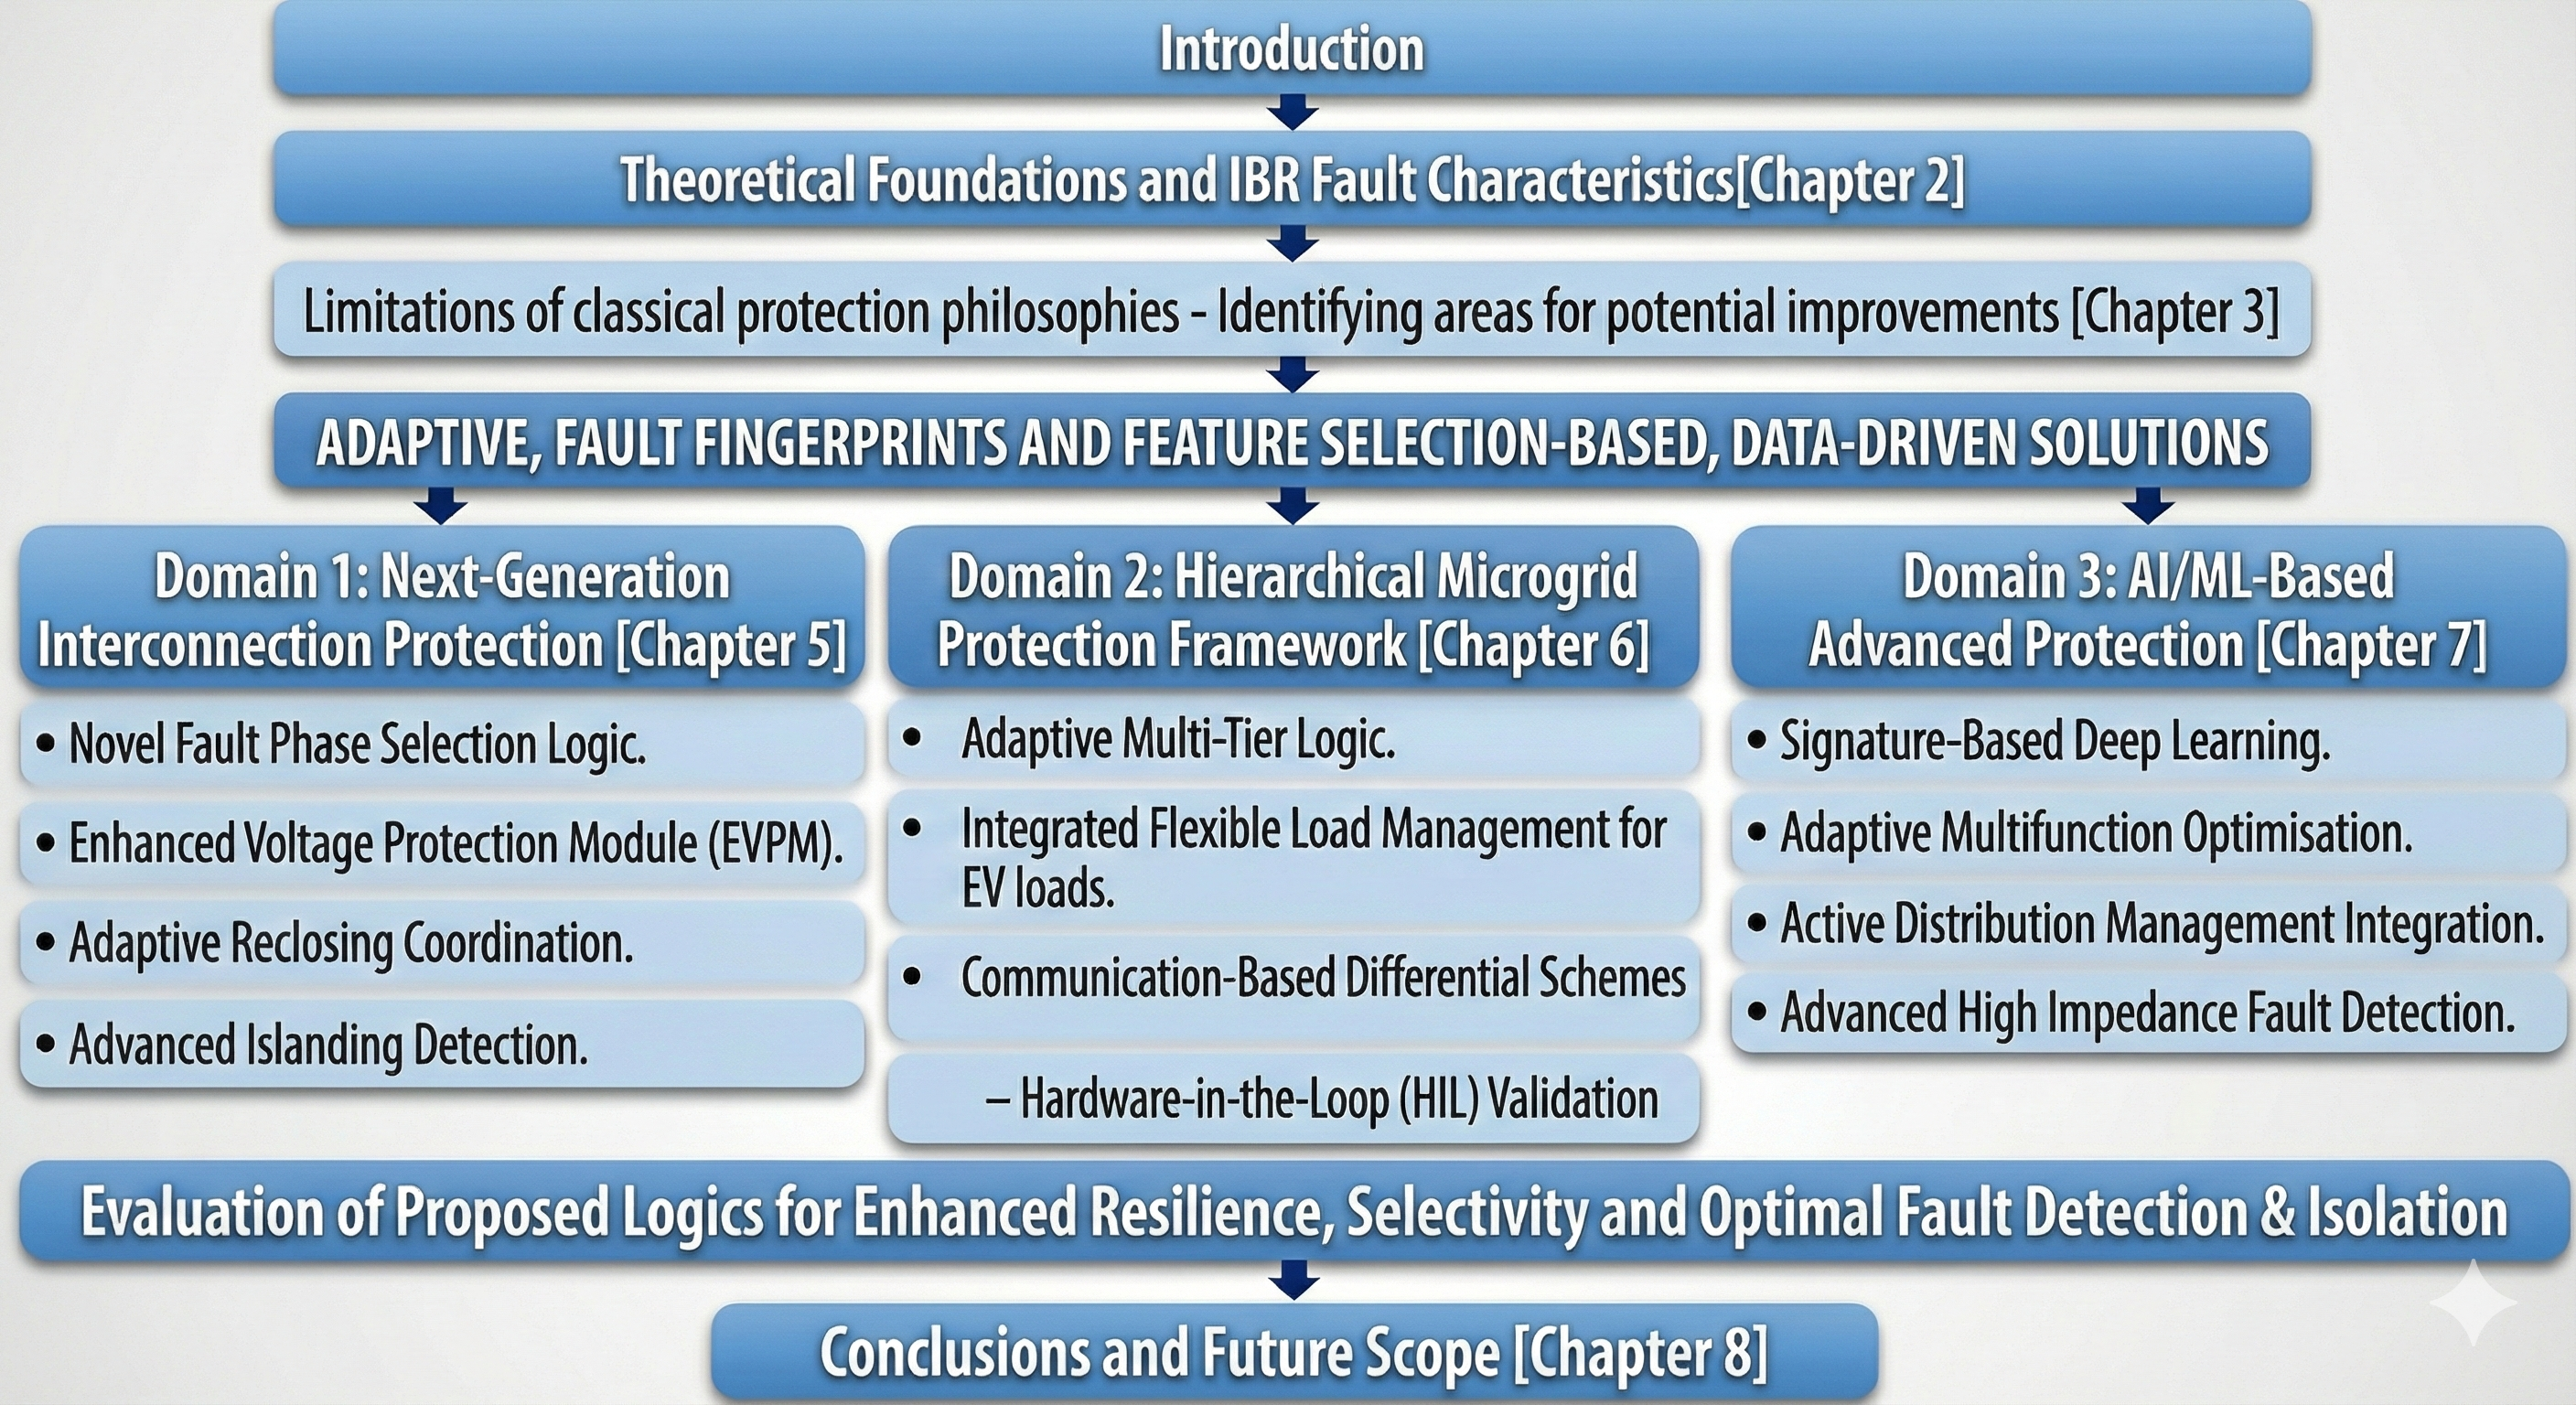
\includegraphics[scale=0.14]{images/chapter_1/ThesisOrganization1.png}
 \caption{Thesis Organization}
\label{ThesisOrganization}
\end{figure}

The remainder of this document is organized as follows:

\begin{itemize}
\item \textbf{Chapter 2: Physics-Informed Modelling of IBRs and Microgrid Dynamics:} Focuses on high-fidelity PSCAD/EMT modeling of PV and Wind sources. Establishes the baseline "fault signatures" required for algorithm development (C1).
% Provides a rigorous mathematical derivation of IBR fault signatures under converter-control constraints. It explores the equivalent circuit formulations of solar PV and Type-III/Type-IV wind turbines, detailing how power electronic control loops, phase-angle manipulation, and grid-code mandated LVRT behaviors actively distort traditional fault signatures.
\item \textbf{Chapter 3: Protection requirements for Active Distribution Networks and Microgrids:} Establishes the research scope, identifies critical gaps in IBR protection, and defines the existential motivation for the study.

% This chapter outlines the existing protection logics and  development of the high-fidelity EMT models for performance evaluations. It details the MATLAB/Simulink environment, the modeling of the active distribution network and microgrid topologies, and the integration of the IEC 61850 GOOSE peer-to-peer communication framework for directional interlocking.
\item \textbf{Chapter 4: Algorithms for Multi -Functional Adaptive Interconnection Protection for IBRs:} Detail the formulation and validation of instantaneous time-domain sampling logics for frequency-independent fault detection.  By rigorous analysis of the simulation data, it benchmarks the performance of the proposed protective algorithms against deterministic legacy relays across a spectrum of extreme operational scenarios, including highly resistive asymmetrical faults, bidirectional infeeds, and dynamic microgrid islanding transitions.

% Introduces instantaneous time-domain sampling and $EVPM$ logic for frequency-independent fault detection. Addressing the critical failure of conventional frequency-dependent RMS measurement windows to distinguish genuine faults during IBR-driven reactive current injection (LVRT mandates), this chapter introduces high-speed instantaneous time-domain sampling at the PCC. By extracting a SPM directly from instantaneous three-phase voltages, the proposed Enhanced Voltage Protection Module (EVPM) dynamically evaluates geometric waveform transformations. This ensures highly selective fault isolation that seamlessly coordinates with IEEE 1547 continuous operation mandates and upstream automatic reclosing schemes. Byrigorous analysis of the simulation data it benchmarks the performance of the proposed protective algorithms against deterministic legacy relays across a spectrum of extreme operational scenarios, including highly resistive asymmetrical faults, bidirectional infeeds, and dynamic microgrid islanding transitions.
\item \textbf{Chapter 5: Adaptive protection architectures for microgrids:} Presents the multi-layered communication-assisted coordination strategy for grid-tied and islanded transitions. Documents the real-time simulation and hardware-in-the-loop results that validate the stability of the proposed schemes under field conditions (C2).


% To mitigate the catastrophic loss of spatial selectivity inherent in traditional protection when microgrids transition between grid-connected and islanded modes—characterized by extreme variances in available fault current—this work proposes a hierarchical, multi-tier protection framework. This architecture actively synthesizes localized voltage-restrained overcurrent elements (ANSI 51V) with ultra-low latency, IEC 61850 GOOSE-based directional interlocking and zone differential schemes to systematically eliminate sympathetic tripping and secure microgrid boundaries regardless of bidirectional power flows.
\item \textbf{Chapter 6: AI/ML-based advanced protection for future microgrid:} Introduces the PINN-based (Physics-Informed Neural Network) architecture for robust fault detection in low-inertia environments.

% Leverages $2\text{-}D$ and $3\text{-}D$ spatial representations via Deep $CNNs$ to transcend deterministic limits. Asserting that the high-noise, transient-heavy fault signatures of heavily penetrated distribution networks outpace the mathematical limitations of deterministic curve-fitting algorithms, this chapter integrates Artificial Intelligence/Machine Learning frameworks for superior fault classification. By processing spatial and transform-domain representations of transients through Deep CNNs, the protection logic autonomously executes dynamic feature selection and optimal settings group modifications, achieving accuracy independent of grid frequency constraints or restricted fault current magnitudes.
\item \textbf{Chapter 7: Conclusion and Future Work:} It concludes by outlining trajectories for future investigations into the integration of machine learning frameworks for autonomous self-healing microgrids.
% The final chapter synthesizes the research findings, highlighting how the proposed architecture successfully resolves the identified research gaps. It concludes by outlining critical avenues for future investigation, including HIL validation and the integration of machine learning frameworks for dynamic threshold optimization.
\end{itemize}


\section{Summary}

This research postulates that the high-density integration of non-synchronous IBRs and the transition toward active microgrid topologies render legacy deterministic protection paradigms—specifically RMS-based overcurrent (ANSI 51), directional (ANSI 67), and distance (ANSI 21) elements—fundamentally obsolete.~Their reliance on fundamental-frequency magnitude sensing introduces an existential susceptibility to protective blinding and catastrophic under-reach when subjected to the non-linear, converter-limited transient signatures of modern networks. Furthermore, these legacy approaches fail to resolve operational conflicts introduced by grid interconnection standards, notably the LVRT and dynamic reactive current injection mandates of IEEE 1547-2018 and IEEE 2800. Consequently, this thesis asserts that securing the resilient grid edge necessitates a transition toward a comprehensive, multi-domain protective architecture that synthesizes magnitude-agnostic instantaneous time-domain signal processing via SPM, hierarchical IEC 61850 GOOSE-enabled peer-to-peer coordination, and Transform-Domain Deep Convolutional Neural Networks (CNNs).~This synthesis guarantees absolute selectivity, sub-cycle response times, and regulatory compliance (IEEE 1547/2800) across extreme topological uncertainties and short-circuit variances.

% 










